\documentclass[11pt]{article}
\usepackage[letterpaper,margin=1in]{geometry}
\usepackage{amsmath,amssymb,amsthm}
\usepackage{graphicx}
\usepackage{xcolor}
\usepackage{hyperref}
\usepackage{microtype}

\hypersetup{colorlinks=true,linkcolor=blue!55!black,urlcolor=blue!55!black,citecolor=blue!55!black}
\newtheorem{theorem}{Theorem}
\newcommand{\B}{\mathbb B}
\newcommand{\C}{\mathbb C}
\newcommand{\id}{\mathop{\rm id}}
\newcommand{\Supp}{\mathop{\rm Supp}}
\newcommand{\Ex}{\mathop{\rm Ex}}

\title{A Boundary-Cap Counterexample to a Support-Point Question for Normal Loewner Chains}
\author{fa\_banach\_001 / agent\_lane\_00}
\date{19 July 2026}

\begin{document}
\maketitle

\noindent\fcolorbox{red!70!black}{red!3}{%
\parbox{0.94\textwidth}{\textbf{Status: candidate counterexample, likely valid.}
Question 3.10 is false as literally printed.  The example is a bounded support
point of $S^0$, but the Herglotz generator of a normal Loewner chain starting
there is uniformly strictly dissipative near a boundary cap of positive
surface measure.}}

\section{Source question}

Bracci and Roth ask the following on PDF page 6 of \emph{Support points and
the Bieberbach conjecture in higher dimension}, arXiv:1603.01532 \cite{BR}.

\begin{figure}[h]
\centering

\includegraphics[width=\textwidth]{figures/open_problem_crop.png}
\caption{Question 3.10 rendered from page 6 of the source paper.}
\end{figure}

In transcription: if a Herglotz vector field $G(z,t)$ generates a normal
Loewner chain $(f_t)$ and
\[
 \limsup_{z\to A}\operatorname{Re}\left\langle
 G(z,t),\frac{z}{\|z\|^2}\right\rangle\le -a
\]
for some $A\subset\partial\B^2$ and almost every $t\ge0$, must
$f_0\notin\Supp(S^0)\cup\Ex(S^0)$?

\section{Definitions}

Let $\B^2$ be the Euclidean unit ball in $\C^2$.  The source uses
\[
 \mathcal M=\{h\in\operatorname{Hol}(\B^2,\C^2):h(0)=0,\ dh_0=\id,
 \ \operatorname{Re}\langle h(z),z\rangle>0\ (z\ne0)\}.
\]
A Herglotz vector field associated with $\mathcal M$ satisfies
$-G(\cdot,t)\in\mathcal M$ almost everywhere.  A normal Loewner chain
has $f_t(0)=0$, $d(f_t)_0=e^t\id$, nested images, and a normal family
$\{e^{-t}f_t\}$.

The compact class $S^0$ consists of normalized univalent maps admitting
parametric representation.  A map $f\in S^0$ is a support point if it
maximizes the real part of a nonconstant continuous linear functional on
$S^0$.

\section{Proof intuition}

The source question imposes strict dissipativity only near \emph{some}
boundary subset.  A support-point generator can lose strict dissipativity at
a small extremal locus while remaining uniformly strict on a large cap away
from that locus.  The sharp quadratic shear already present in the source
does exactly this.

Its coefficient is chosen so that the generator is barely admissible: the
dissipativity expression reaches zero at the points maximizing
$|z_1||z_2|^2$.  Near the coordinate circle $z_2=0$, however, the same
expression is close to $-1$.  A fixed cap around that circle therefore meets
the hypothesis, even though the initial shear is detected as a support point
by the sharp coefficient functional.

\section{Counterexample}

Set
\[
 c=\frac{3\sqrt3}{2},\qquad
 \Phi(z_1,z_2)=(z_1+c z_2^2,z_2),\qquad
 f_t=e^t\Phi,
\]
and define the autonomous field
\begin{equation}\label{eq:G}
 G(z_1,z_2)=(-z_1+c z_2^2,-z_2).
\end{equation}

\begin{theorem}
The family $(f_t)_{t\ge0}$ is a normal Loewner chain generated by $G$,
and $f_0=\Phi$ belongs to $\Supp(S^0)$.  Nevertheless, with
\[
 A=\{\zeta\in\partial\B^2:|\zeta_2|\le1/4\}
\]
one has
\[
 \limsup_{z\to A}\operatorname{Re}\left\langle
 G(z,t),\frac{z}{\|z\|^2}\right\rangle\le-\frac34
\]
for every $t\ge0$.  Hence this is a counterexample to Question 3.10.
\end{theorem}

\begin{proof}
\textbf{Step 1: the field is admissible.}
Write $r=\|z\|$, $x=|z_1|$, and $y=|z_2|$.  Elementary one-variable
optimization gives
\begin{equation}\label{eq:max}
 \max_{x^2+y^2=r^2}xy^2=\frac{2r^3}{3\sqrt3}.
\end{equation}
Consequently, for $0<r<1$,
\[
 \operatorname{Re}\langle-G(z),z\rangle
 =r^2-c\operatorname{Re}(z_2^2\overline{z_1})
 \ge r^2-cxy^2\ge r^2-r^3>0.
\]
Also $-G(0)=0$ and $d(-G)_0=\id$.  Thus $-G\in\mathcal M$.

\textbf{Step 2: the normal chain.}
The Jacobian of $\Phi$ is
\[
 d\Phi_z=\begin{pmatrix}1&2cz_2\\0&1\end{pmatrix},
\]
and direct multiplication using \eqref{eq:G} gives
$d\Phi_zG(z)=-\Phi(z)$.  Therefore
\[
 \frac{\partial f_t}{\partial t}(z)=f_t(z)=-d(f_t)_zG(z),
\]
so $(f_t)$ solves the Loewner--Kufarev PDE.  Each $f_t$ is an entire
univalent triangular map, and $\{e^{-t}f_t\}=\{\Phi\}$ is normal.
The standard Loewner existence/subordination theorem quoted in the source
therefore makes $(f_t)$ a normal Loewner chain.  In particular,
$\Phi=f_0\in S^0$.

\textbf{Step 3: $\Phi$ is a support point.}
We include the short coefficient argument used in the source.  If
$f\in S^0$ has coefficient $b^1_{0,2}$ and is represented by a Herglotz
field with coefficient $q^1_{0,2}(t)$, the degree-two evolution equation has
no lower-degree remainder and yields
\begin{equation}\label{eq:coeff}
 b^1_{0,2}(f)=\int_0^\infty e^{-t}q^1_{0,2}(t)\,dt.
\end{equation}
Harmonic decoupling preserves the field
\[
 (-z_1+q^1_{0,2}(t)z_2^2,-z_2).
\]
Its admissibility, together with \eqref{eq:max} at $r=1$, implies
\[
 |q^1_{0,2}(t)|\le\frac{3\sqrt3}{2}=c
\]
for almost every $t$.  Equation \eqref{eq:coeff} gives
$|b^1_{0,2}(f)|\le c$.  The continuous coefficient functional is not
constant on $S^0$, and $b^1_{0,2}(\Phi)=c$.  Hence $\Phi$ maximizes its
real part and belongs to $\Supp(S^0)$.

\textbf{Step 4: strict dissipation on a boundary cap.}
For $z\ne0$,
\begin{equation}\label{eq:diss}
 \operatorname{Re}\left\langle G(z),\frac{z}{\|z\|^2}\right\rangle
 =-1+c\frac{\operatorname{Re}(z_2^2\overline{z_1})}{\|z\|^2}.
\end{equation}
The set $A$ is a nonempty closed cap with nonempty relative interior and
positive surface measure.  Passing to $A$ in \eqref{eq:diss} gives
\[
 \limsup_{z\to A}\operatorname{Re}\left\langle
 G(z),\frac{z}{\|z\|^2}\right\rangle
 \le -1+c\sup_{\zeta\in A}|\zeta_1||\zeta_2|^2
 \le -1+\frac{c}{16}
 =-1+\frac{3\sqrt3}{32}< -\frac34.
\]
Because $G$ is autonomous, this holds at every time.  The hypothesis of
Question 3.10 is satisfied with $a=3/4$, but its conclusion is false since
$f_0=\Phi\in\Supp(S^0)$.
\end{proof}

\begin{figure}[ht]
\centering
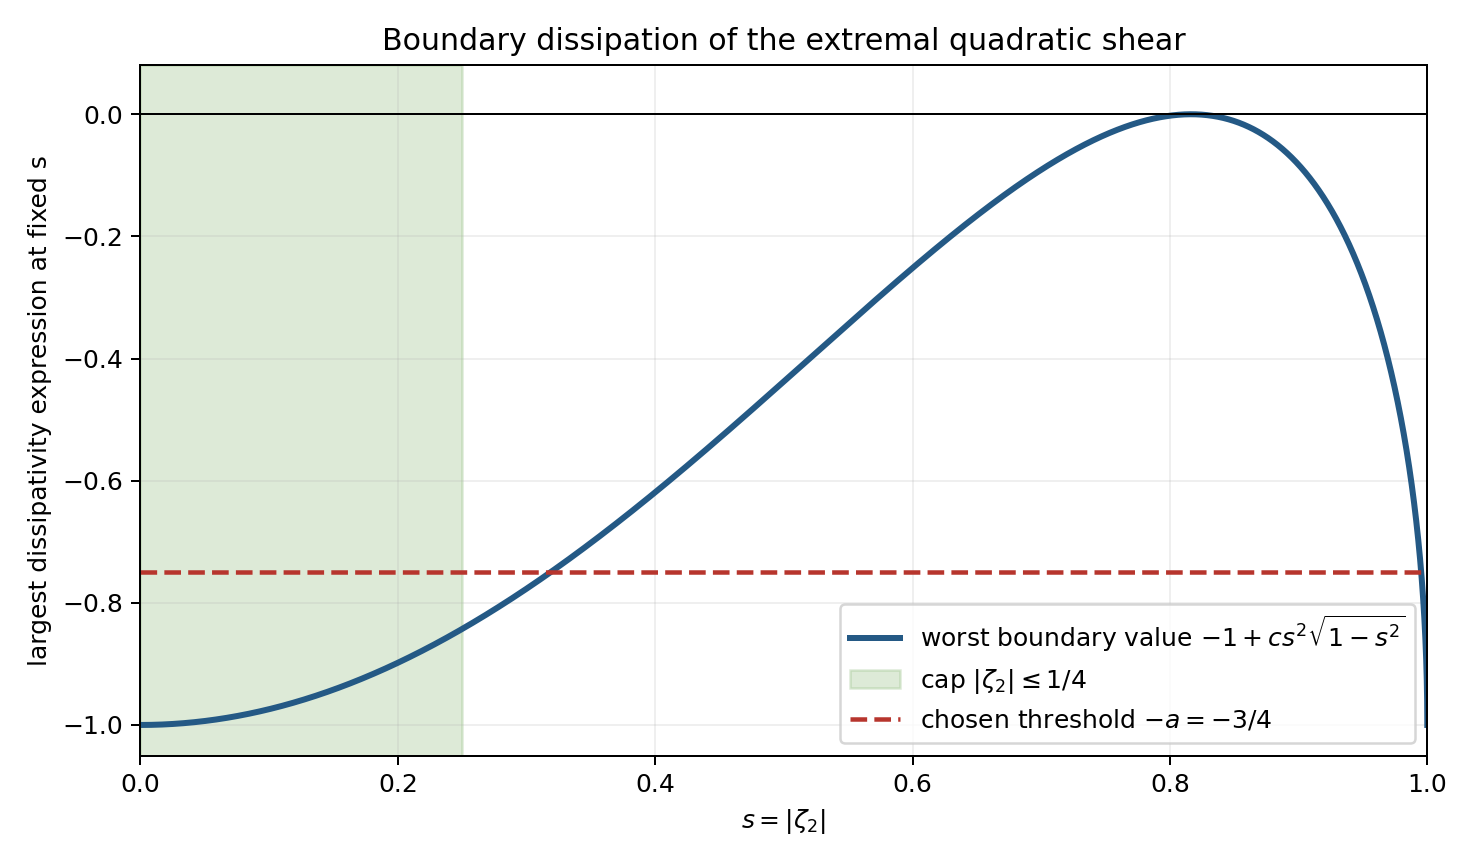
\includegraphics[width=0.86\textwidth]{figures/boundary_dissipativity.png}
\caption{The worst boundary value at fixed $|\zeta_2|$.  The green cap lies
strictly below the chosen threshold $-3/4$.}
\end{figure}

\section{Verification}

The script \texttt{code/verify\_counterexample.py} samples the exact
one-variable maximization, checks the Loewner PDE identity at complex points,
integrates the degree-two coefficient kernel, and generates the figure.  It
reports the exact extremal product to numerical precision, a zero PDE
residual, a cap supremum below $-3/4$, and \texttt{PASS}.  Full commands and
output are recorded in \texttt{verification.md}; computation is not used as
proof.

\section{Scope and bounded novelty check}

The theorem disproves Question 3.10 as printed, specifically its phrase
``for some $A\subset\partial\B^2$.''  It does not address a strengthened
question requiring $A=\partial\B^2$, or an unprinted largeness or global
accessibility condition.

The run indexes were searched by arXiv id, title, question number, and core
terms.  A bounded primary-source web/arXiv search used the exact question
language, author names, ``exponentially squeezing,'' and the constant
$3\sqrt3/2$.  It found the source and nearby Loewner work but no later explicit
resolution or matching cap counterexample.  This is a bounded search, not an
exhaustive novelty claim.

\section{Human-review recommendation}

Independent review should focus on the intended semantics of
$\limsup_{z\to A}$ and whether the authors silently intended a stronger
hypothesis on $A$.  Under the literal printed statement, the cap used here is
substantial: it has positive surface measure and nonempty relative interior.
The algebraic and coefficient checks are otherwise elementary and explicit.

\begin{thebibliography}{9}
\bibitem{BR}
F. Bracci and O. Roth,
\emph{Support points and the Bieberbach conjecture in higher dimension},
Complex Analysis and Dynamical Systems, Trends in Mathematics,
Birkh\"auser/Springer (2018), 67--79; arXiv:1603.01532.
\end{thebibliography}

\end{document}
